\documentclass[12pt]{article}
\usepackage[dvips]{graphicx}
\title{A Business Rule Extension Framework Proposal}
\author{Leo Przybylski}

\begin{document}
  \maketitle
  \tableofcontents

  \begin{abstract}
To manage \emph{business objects} appropriately, a set of rules --
\emph{business rules} -- are applied. A business rule is an acceptable use
case scenario that describes the intended behavior of a 
\emph{business object}. One goal of the Kuali API is to offer,
extension of it through the creation of \emph{business objects}; likewise,
\emph{business rules} may be required to handle additional 
\emph{business objects}. 

The role of a \emph{business object} deterimines the rule(s) that are to be
applied. The \sf \verb|TransactionalDocument| \rm is the most interesting
\emph{business object} in the scope of this document.

A set of business rules are defined for a \sf \verb|TransactionalDocument|. \rm
Base rules packaged with the Kuali Project API may fulfill the needs of some 
institutions; however, it is not expected that the base rules are adequate for
every institution or for all requirements of the application. Some 
institutions may have a proprietary set of rules to be applied to existing
\sf \verb|TransactionalDocument| \rm \emph{business objects} to support
new or existing \emph{business rules}. 

It has been decided that a framework to support creation of or modification of
arbitrary \emph{business rules} without require special maintenance of Kuali
project source code is necessary.
  \end{abstract}
  \section{Introduction}
When an institution desires to create third-party business rules for any reason,
 the available framework is expected to support the creation regardless of the 
complexity. This flexibility comes from isolating the business rules from the 
Kuali API save two interfaces (\sf \verb|PolicyFactory |\rm and \sf 
\verb| Policy|\rm .) 

The aforementioned flexibility allows arbitrary business rule definitions 
to be implemented without the need for proprietary code modifications. To
summarize, the beneficial characteristics of the framework are:
\begin{itemize}
  \item Allow arbitrary class definitions implementing the 
  \sf Policy \rm interface.
  \item Delegate constructor and method calls, so the framework will 
  automatically instantiate \sf Policy \rm implementations.
  \item Allow \sf Policy \rm implementations proper access to 
  \sf TransactionalDocument \rm instances.
  \item \sf Policy \rm implementations can be maintained independently of
  Kuali API.
\end{itemize}
\begin{quote}
...a structure such
that it is easy to process arbitrary business rules against a document,
while making it easy for local implementations (ie, specific schools) to
replace the reference implementation's business rules with their own
without requiring customization of the reference application.  In other
words, pain should be absolutely minimal to re-attach local business
rules...  - Andrew Hollamon
\end{quote}

  \section{Use Cases}
  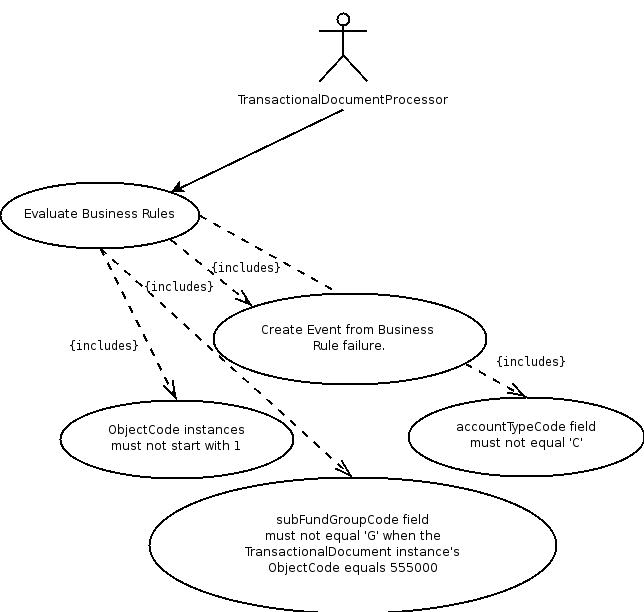
\includegraphics[scale=0.35]{Diagrams/UseCases.eps}  \\

\emph{Business rules} are acceptable use case scenarios for
\emph{business objects}. When \emph{business objects} don't play by the rules,
they are following exceptional use case scenarios rather than the rules
intended. Above is a diagram describing use cases followed in the examples
of this proposal. 

  \section{Framework Overview}
  \subsection{The Framework Structure}
  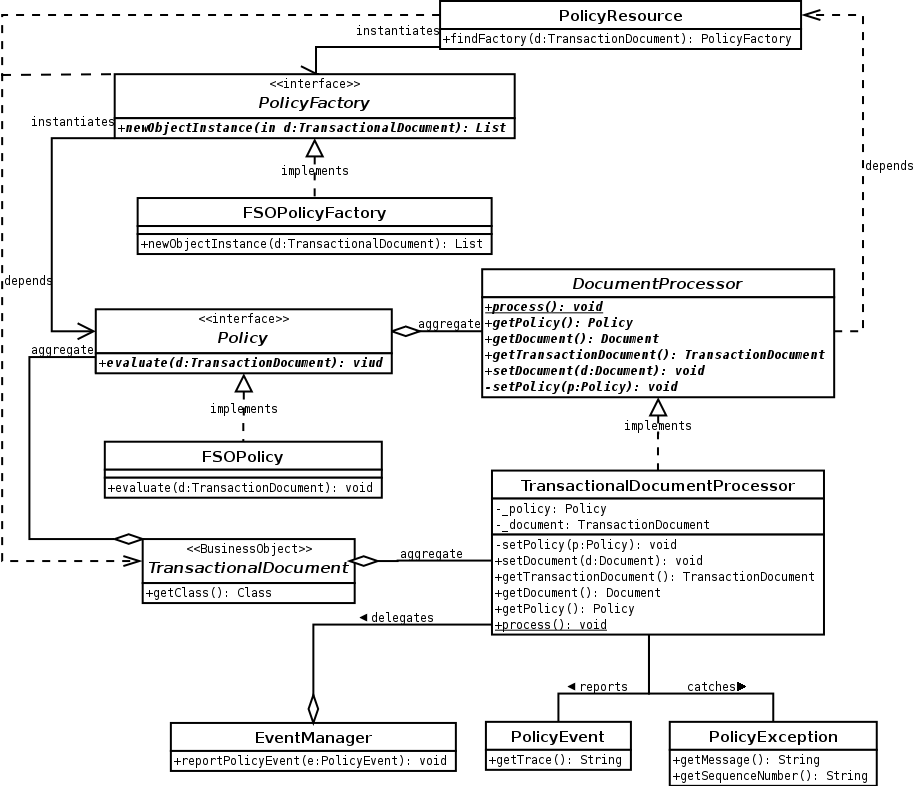
\includegraphics[scale=0.35]{Diagrams/Service_Class.eps} \\

  Illustrated above is a high-level view of class relationships used in the
extension framework. With each use of the \sf FactoryClass \rm pattern, a new
level of flexibility and complexity is added. 
 
For example, mapping a single \sf Policy \rm
to a \sf TransactionalDocument \rm may have been sufficient for some 
applications, but the use of multiple \sf Policy \rm instances adds more 
flexibility by allowing the reuse of \sf Policy \rm definitions. The cost is
that implementation of this kind of flexibility required the use of a 
\sf PolicyFactory \rm abstraction that allows dynamic creation/discovery of
\sf Policy \rm definitions. Also, discovery of the \sf PolicyFactory \rm
was handled by mapping it to a \sf TransactionalDocument \rm definition just
as the \sf Policy \rm is. \\

  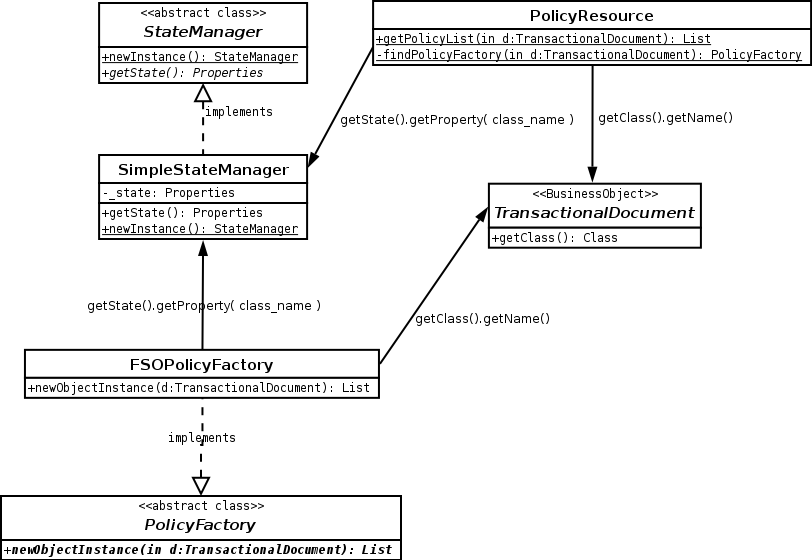
\includegraphics[scale=0.35]{Diagrams/StateManager_class.eps} \\

  Above is a view that illustrates the relationship between \sf Policy\rm,
\sf PolicyFactory\rm, \sf TransactionalDocument\rm, and \sf StateManager\rm
, which is used to persistently store the mappings. 

The \sf PolicyResource \rm queries the \sf StateManager \rm using the fully 
qualified class name of the \sf TransactionalDocument\rm. Let's say for example,
the name is \sf InternalBillingDocument\rm. The \sf StateManager \rm answers
with the class name of the mapped \sf PolicyFactory\rm. \sf PolicyFactory \rm
applies the same pattern to discovering the appropriate \sf Policy \rm 
instances. 

When all the \sf Policy \rm definitions have been discovered, then all the
business rules can be applied by the \sf TransactionalDocumentProcessor\rm. 
The functionality of the \sf Policy \rm definition is transparent to the 
\sf TransactionalDocument \rm and the \sf TransactionalDocumentProcessor \rm
instances which allows arbitrary business rules to be applied to whatever
\sf TransactionalDocument\rm.

\subsubsection{When They Don't Play by the Rules...}
A failure to comply with business rules is considered an exceptional use case,
 and results in an invocation of the Event Sub-System. A discussion on the Event
 Sub-System in its entirety is beyond the scope of this proposal; however, a 
general abstraction can be explained. \\

  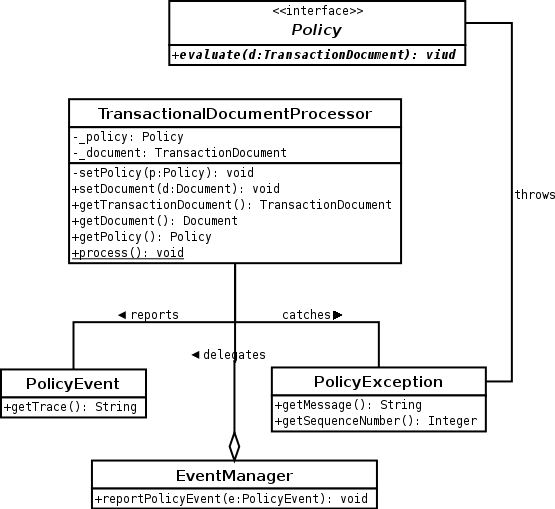
\includegraphics[scale=0.45]{Diagrams/PolicyEvents_class.eps} \\

To invoke the Event Sub-System, an implementation of \sf Policy\rm, or 
\sf PolicyFactory throws \rm a \sf PolicyException\rm. The 
\sf PolicyException \rm is
part of an Event Sub-System. It is used to create an \sf PolicyEvent \rm which
is handled by the Event Sub-System. When the \sf TransactionalDocumentProcessor 
\rm catches a \sf PolicyException\rm, it assumes they have all are a result
of business rule violations and throws an \sf Error \rm back to its caller after
reporting the \sf PolicyEvent\rm. What happens after the \sf PolicyEvent \rm is
reported is up to the implementation of the system. It may log \sf PolcyEvent
\rm instances in a database, a flat file, or just in memory.

Such a system adds further flexibility to the framework for 
managing business objects by logging and coordinating their behavior with
business rules. It is easier to analyze \emph{business rules} for better design
and also in the debugging/troubleshooting of the \sf Policy \rm implementation.

The following constrains the Event Sub-System:
\begin{itemize}
\item \sf PolicyException \rm must be thrown by \sf evaluate() \rm method of 
any \sf Policy \rm implementation.
\item Is always caught by the calling \sf TransactionalDocumentProcessor \rm
instance.
\item Provides a \sf sequenceNumber \rm of the \sf AccountingLine \rm that
caused the \emph{business rule} evaluation failure.
\item \sf EventManager \rm must handle \sf PolicyEvent \rm instances.
\item \sf PolicyEvent \rm can only be instantiated from a \sf PolicyException\rm.
\end{itemize}

  Process flow regarding order of operations and intantiation of objects are
explained in greater detail in the following section. \\

  \subsubsection{Framework Integration with the Existing API}

  The framework integrates through a single interface in the existing API, the
\sf TransactionalDocument \rm interface. The \sf TransactionalDocument \rm 
interface can be implemented and polymorphically used by the
\sf TransactionalDocumentProcessor \rm to discover and evaluate \sf Policy \rm
instances relating the \sf TransactionalDocument\rm.

See the section on \emph{Creating the Implementation} for more information. 

  \subsection{Sequence or Process Flow}

  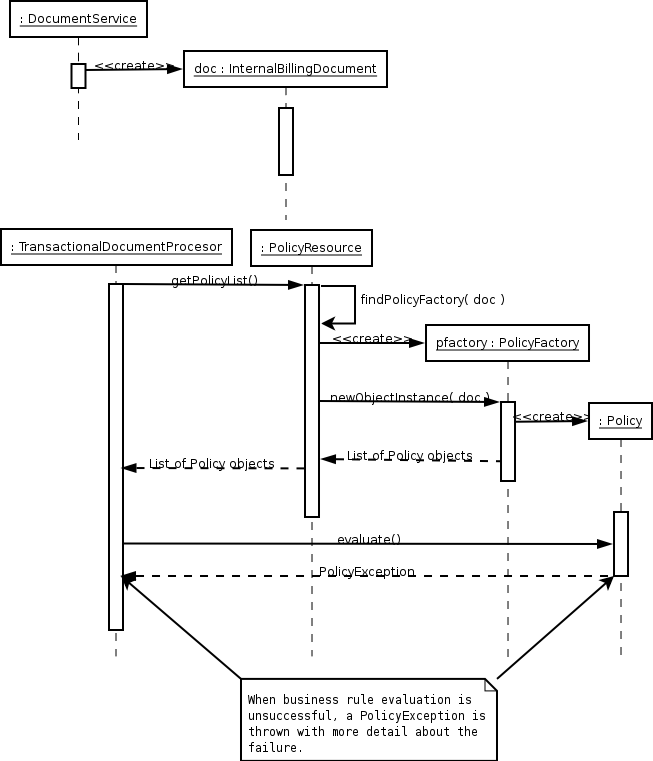
\includegraphics[scale=0.45]{Diagrams/DocumentProcessor_Sequence.eps} \\

  Above is in illustration of the order of operations in sequence. This is a
high-level diagram and omits information about how the mappings are accessed. 
The process of discovering \sf Policy \rm definitions or
\sf PolicyFactory \rm definitions from the mappings is illustrated in the next
diagram along with discussion. \\

  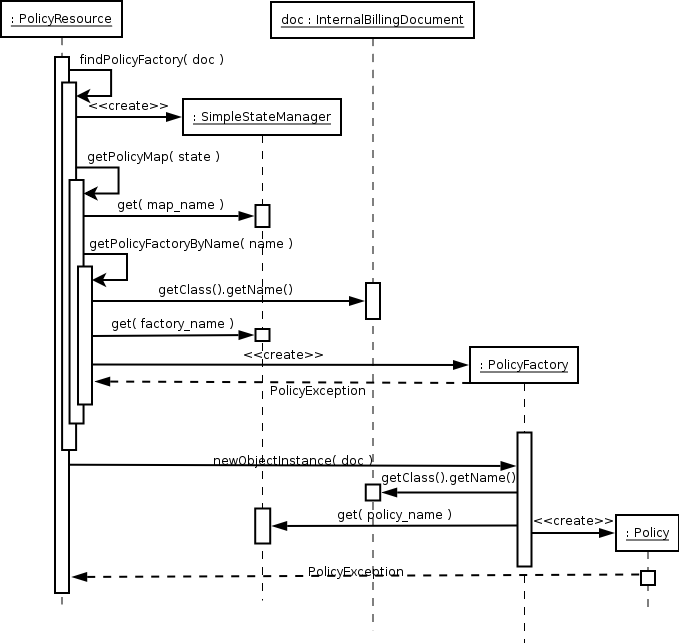
\includegraphics[scale=0.45]{Diagrams/Mapping_Sequence.eps} \\

  Here the aforementioned relationships from the second diagram in 
the \emph{Framework Overview} are realized in a time-ordered diagram.

  \section{Creating the Implementation}
  There are three interfaces part of the framework implementation:
\begin{description}
  \item[Map] is required to provide an implementation that maps a 
\sf TransactionalDocument \rm implementation to a \sf Policy \rm or
 \sf PolicyFactory \rm implementation.
  \item[PolicyFactory] is used to create a \sf Policy \rm collection from
information provided in the \sf Map\rm.
  \item[Policy] is the main \emph{business rule} context. It is responsible
for evaluating \emph{business rules}.
\end{description}
  \subsection{Map of Policy Implementations}
  For the purpose of this proposal, an example \sf Map \rm implementation is
provided. The implementation is acquired from the \sf StateManager \rm
instance \sf by an instance of \sf PolicyResource \rm (see the section on
\emph{Process Flow} for more information.) The 
\sf StateManager \rm queries a \sf System \rm property \sf kuali.map.class \rm
to identify the \sf Map \rm implementation. Observe the following sample 
source from \sf PolicyResource \rm that describes how the \sf Map \rm is
acquired from the \sf StateManager\rm: 
  \sf \begin{verbatim} 
    return ( Map )Class
            .forName( state.get( MAP_STRING ).toString() )
            .newInstance();
...
...
    private static final String MAP_STRING = "kuali.map.class";

  \end{verbatim} \rm 

  Any \sf Map \rm implementation will work (\sf SynchronizedMap\rm,
 \sf HashMap\rm, etc...) The example provided, makes use of the
 \sf SimpleStateManager \rm implementation as a \sf Map\rm, but that is not
necessary.
  \subsection{PolicyFactory}
  \sf PolicyFactory \rm is responsible for building a \sf Collection \rm
of the correct \sf Policy \rm instances for the specified 
\sf TransactionalDocument\rm. \sf PolicyFactory \rm implementations are 
mapped directly to \sf TransactionalDocument\rm class names. The example
 implementation provided with the proposal obtains the \sf Map \rm 
implementation from a \sf StateManager \rm instance, and queries the 
\sf Map \rm implementation using the \sf TransactionalDocument \rm class
name for the mapped \sf PolicyFactory\rm. Observe the following sample
source from \sf PolicyResource \rm that describes the \sf PolicyFactory \rm
class name is queried from the \sf Map\rm:
  \sf \begin{verbatim}
     return policy_map.get( FACTORY_PREFIX
                            + d.getClass().getName() ).toString();
...
...
private static final String FACTORY_PREFIX = "kuali.map.factory.";
  \end{verbatim} \rm

  The mapping uses a prefix of \sf kuali.map.factory. \rm to distinguish 
itself from \sf Policy \rm mappings.

   The example provided with this proposal is
 \sf org.kuali.bo.FSOPolicyFactory\rm. 
To create an implementation class definition for the \sf PolicyFactory \rm 
abstraction,
the following was done to create \sf FSOPolicyFactory\rm:
\begin{enumerate}
  \item Extend the \sf PolicyFactory \rm abstract class.
  \sf \begin{verbatim}
  public class FSOPolicyFactory extends PolicyFactory {
  \end{verbatim} \rm
  \item Override the \sf getObjectInstance \rm method.
  \sf \begin{verbatim}
    public Object getObjectInstance( TransactionalDocument d )
        throws Exception {
        // The purpose behind the factory is flexibility with
        // assigning Policy implementations to a
        // TransactionalDocument.

        // There is already a mapping to the PolicyFactory from 
        // the TransactionalDocument, so another mapping isn't
        // necessary. It is possible to just add object 
        // instantiations here without losing any flexibility at 
        // all. For example, the following is possible:

        List retval = new ArrayList();
        retval.add( new FSOPolicy( d ) );
        // retval.add( new FSOInternalBillingPolicy( d ) );
        // retval.add( new FSOPayrollPolicy( d ) );
        return retval;

        // It is just EXTRA flexibility to reuse the 
        // mapping interface.
    }
  \end{verbatim} \rm
\end{enumerate}


  \subsection{Policy}
A \sf Policy \rm implementation is a class definition of a \emph{business rule}.
 With each \sf Policy \rm instance that is evaluated by a 
\sf TransactionalDocumentProcessor\rm, a new \emph{business rule} is 
evaluated against a \sf TransactionalDocument\rm. 

   The example provided with this proposal is \sf org.kuali.bo.FSOPolicy\rm.
To create an implentation class definition for the \sf Policy \rm interface,
the following was done to create \sf FSOPolicy\rm:
\begin{enumerate}
  \item Implement \sf Policy \rm.
  \sf \begin{verbatim}
    public class FSOPolicy implements Policy {
  \end{verbatim} \rm

  \item Override the \sf evaluate \rm method (this is probably the most
important part of \sf Policy\rm.)
  \sf \begin{verbatim}
    public void evaluate() throws Throwable {
        InternalBillingDocument doc =
                ( InternalBillingDocument )getDocument();
        AccountingLine actl = null;
        for( Iterator line_it = doc.sourceAccountingLines();
             line_it.hasNext(); actl = line_it.next() ) {
            if( actl.getObjectCode()
                    .toString().startsWith( "1" ) ) {
                throw new PolicyException
                        ( BAD_OBJECT_CODE_MESSAGE);
            }
            if( actl.getAccount()
                    .getAccountTypeCode().equals( "C" ) ) {
                throw new PolicyException
                        ( BAD_ACCOUNT_TYPE_MESSAGE );
            }
            if( actl.getAccount().getSubFundGroupCode()
                    .equals( "G" ) &&
                actl.getObjectCode()
                    .toString().equals( "555000" ) ) {
                throw new PolicyException
                        ( BAD_GROUP_CODE_MESSAGE );
            }
        }
    }
  \end{verbatim} \rm

  \item Override the \sf getDocument \rm and \sf setDocument \rm methods.
  \sf \begin{verbatim}
    private void setDocument( TransactionalDocument d ) { 
        _document = d; 
    }

    public TransactionalDocument getDocument() {  
        return _document; 
    }

    private TransactionalDocument _document
  \end{verbatim} \rm

\end{enumerate}

\section{Invoking the Implementation}
 \sf TransactionalDocumentProcessor \rm manages the \emph{business rules}. All
that is required obtaining a \sf TransactionalDocument \rm for the \sf
TransactionalDocumentProcessor to handle\rm.

  \sf \begin{verbatim}
  try {
      new TransactionalDocumentProcessor
              ( SomeDocumentService.getNewDocument
                      ( "org.kuali.bo.InternalBillingDocument" ) )
              .process();
  } catch( Error e ) {
     // Do something 
  }
  \end{verbatim} \rm

  The above creates a new \sf InternalBillingDocument \rm instance and a 
new \sf TransactionalDocumentProcessor\rm. Finally, it invokes \sf process() \rm
method and tries to catch the \sf Error \rm if there is one.

\end{document}
